\documentclass[11pt,a4paper]{article}
%%%%%%%%%%%%%%%%%%%%%%%%%%%%%%%%%%%%%%%%%%%%%%%%%%%%%%%%
%                      PACKAGES                        %
%%%%%%%%%%%%%%%%%%%%%%%%%%%%%%%%%%%%%%%%%%%%%%%%%%%%%%%%

\usepackage[utf8]{inputenc}
\usepackage{graphicx} % Allows you to insert figures
\usepackage[export]{adjustbox}
\usepackage{booktabs}
\usepackage{amsmath} % Allows you to do equations
\usepackage{helvet}
\usepackage{hyperref}
\renewcommand{\familydefault}{\sfdefault}
\usepackage[a4paper, total={6.5in, 9.5in}]{geometry} % Formats the paper size, orientation, and margins
\linespread{1.1} % about 1.5 spacing in Word
\setlength{\parindent}{0pt} % no paragraph indents
\setlength{\parskip}{1em} % paragraphs separated by one line
\usepackage{listings}
\usepackage{enumitem}
\usepackage{xcolor}
\usepackage{hyperref}
\hypersetup{
	colorlinks=true,
	urlcolor=cyan,
	linktoc=none,
}
\usepackage{fancyhdr}
\pagestyle{fancy}
\fancyhead[L,C,R]{}
\fancyfoot[L]{Blix - AI Photo Editor}
\fancyfoot[C]{}
\fancyfoot[R]{\textbf{\thepage}}
\renewcommand{\headrulewidth}{0pt}
\renewcommand{\footrulewidth}{0.5pt}

\definecolor{codegreen}{rgb}{0,0.6,0}
\definecolor{codegray}{rgb}{0.5,0.5,0.5}
\definecolor{codepurple}{rgb}{0.58,0,0.82}
\definecolor{backcolour}{rgb}{0.95,0.95,0.92}

\lstdefinestyle{mystyle}{
backgroundcolor=\color{backcolour},
commentstyle=\color{codegreen},
keywordstyle=\color{magenta},
numberstyle=\tiny\color{codegray},
stringstyle=\color{codepurple},
basicstyle=\ttfamily\footnotesize,
breakatwhitespace=false,
breaklines=true,
keepspaces=true,
numbersep=5pt,
showspaces=false,
showstringspaces=false,
showtabs=false,
tabsize=2,
}

\lstset{style=mystyle}
\def\code#1{\texttt{#1}}

%%%%%%%%%%%%%%%%%%%%%%%%%%%%%%%%%%%%%%%%%%%%%%%%%%%%%%%%
%            TITLE PAGE & TABLE OF CONTENTS            %
%%%%%%%%%%%%%%%%%%%%%%%%%%%%%%%%%%%%%%%%%%%%%%%%%%%%%%%%

\begin{document}

\begin{titlepage}
	\centering
    % \includegraphics[width=0.5\textwidth]{your_logo.png}\par\vspace{1cm}
    {\scshape\LARGE Technical Installation Manual\par}
    \vspace{1.5cm}
    {\huge\bfseries Blix - AI Photo Editor\par}
    \begin{figure}[h]
        \centering % center the image
        \includegraphics[width=0.5\textwidth]{../pics/blix.png}
    \end{figure}
    \vspace{2.5cm}
    {\Large\itshape The Spanish Inquisition\par}
	\begin{tabular}{|c|c|}
		\hline
		\textbf{Name} 		& \textbf{Student Number} \\
		\hline
		Armand Krynauw		& u04868286  \\
		Jake Mileham		& u21692492  \\
		Dino Gironi			& u21630276  \\
		Karel Olwage		& u21555258  \\
		Francois Combrinck	& u21729752  \\
		\hline
	\end{tabular}
    \vfill
    {\large \today\par}
\end{titlepage}

\tableofcontents
\pagebreak

%%%%%%%%%%%%%%%%%%%%%%%%%%%%%%%%%%%%%%%%%%%%%%%%%%%%%%%%
%                MAIN DOCUMENT CONTENT                 %
%%%%%%%%%%%%%%%%%%%%%%%%%%%%%%%%%%%%%%%%%%%%%%%%%%%%%%%%

\addcontentsline{toc}{section}{Introduction}
\section*{Introduction}

Blix is a native cross-platform desktop application designed to provide users
with a powerful and intuitive photo editing experience.

\addcontentsline{toc}{section}{General Installation}
\section*{General Installation}

Download the packaged app from our GitHub release page by using the following 
	\href{https://github.com/COS301-SE-2023/AI-Photo-Editor/releases/tag/v1.0.0}{link}.
\begin{figure}[ht]
	\centering
	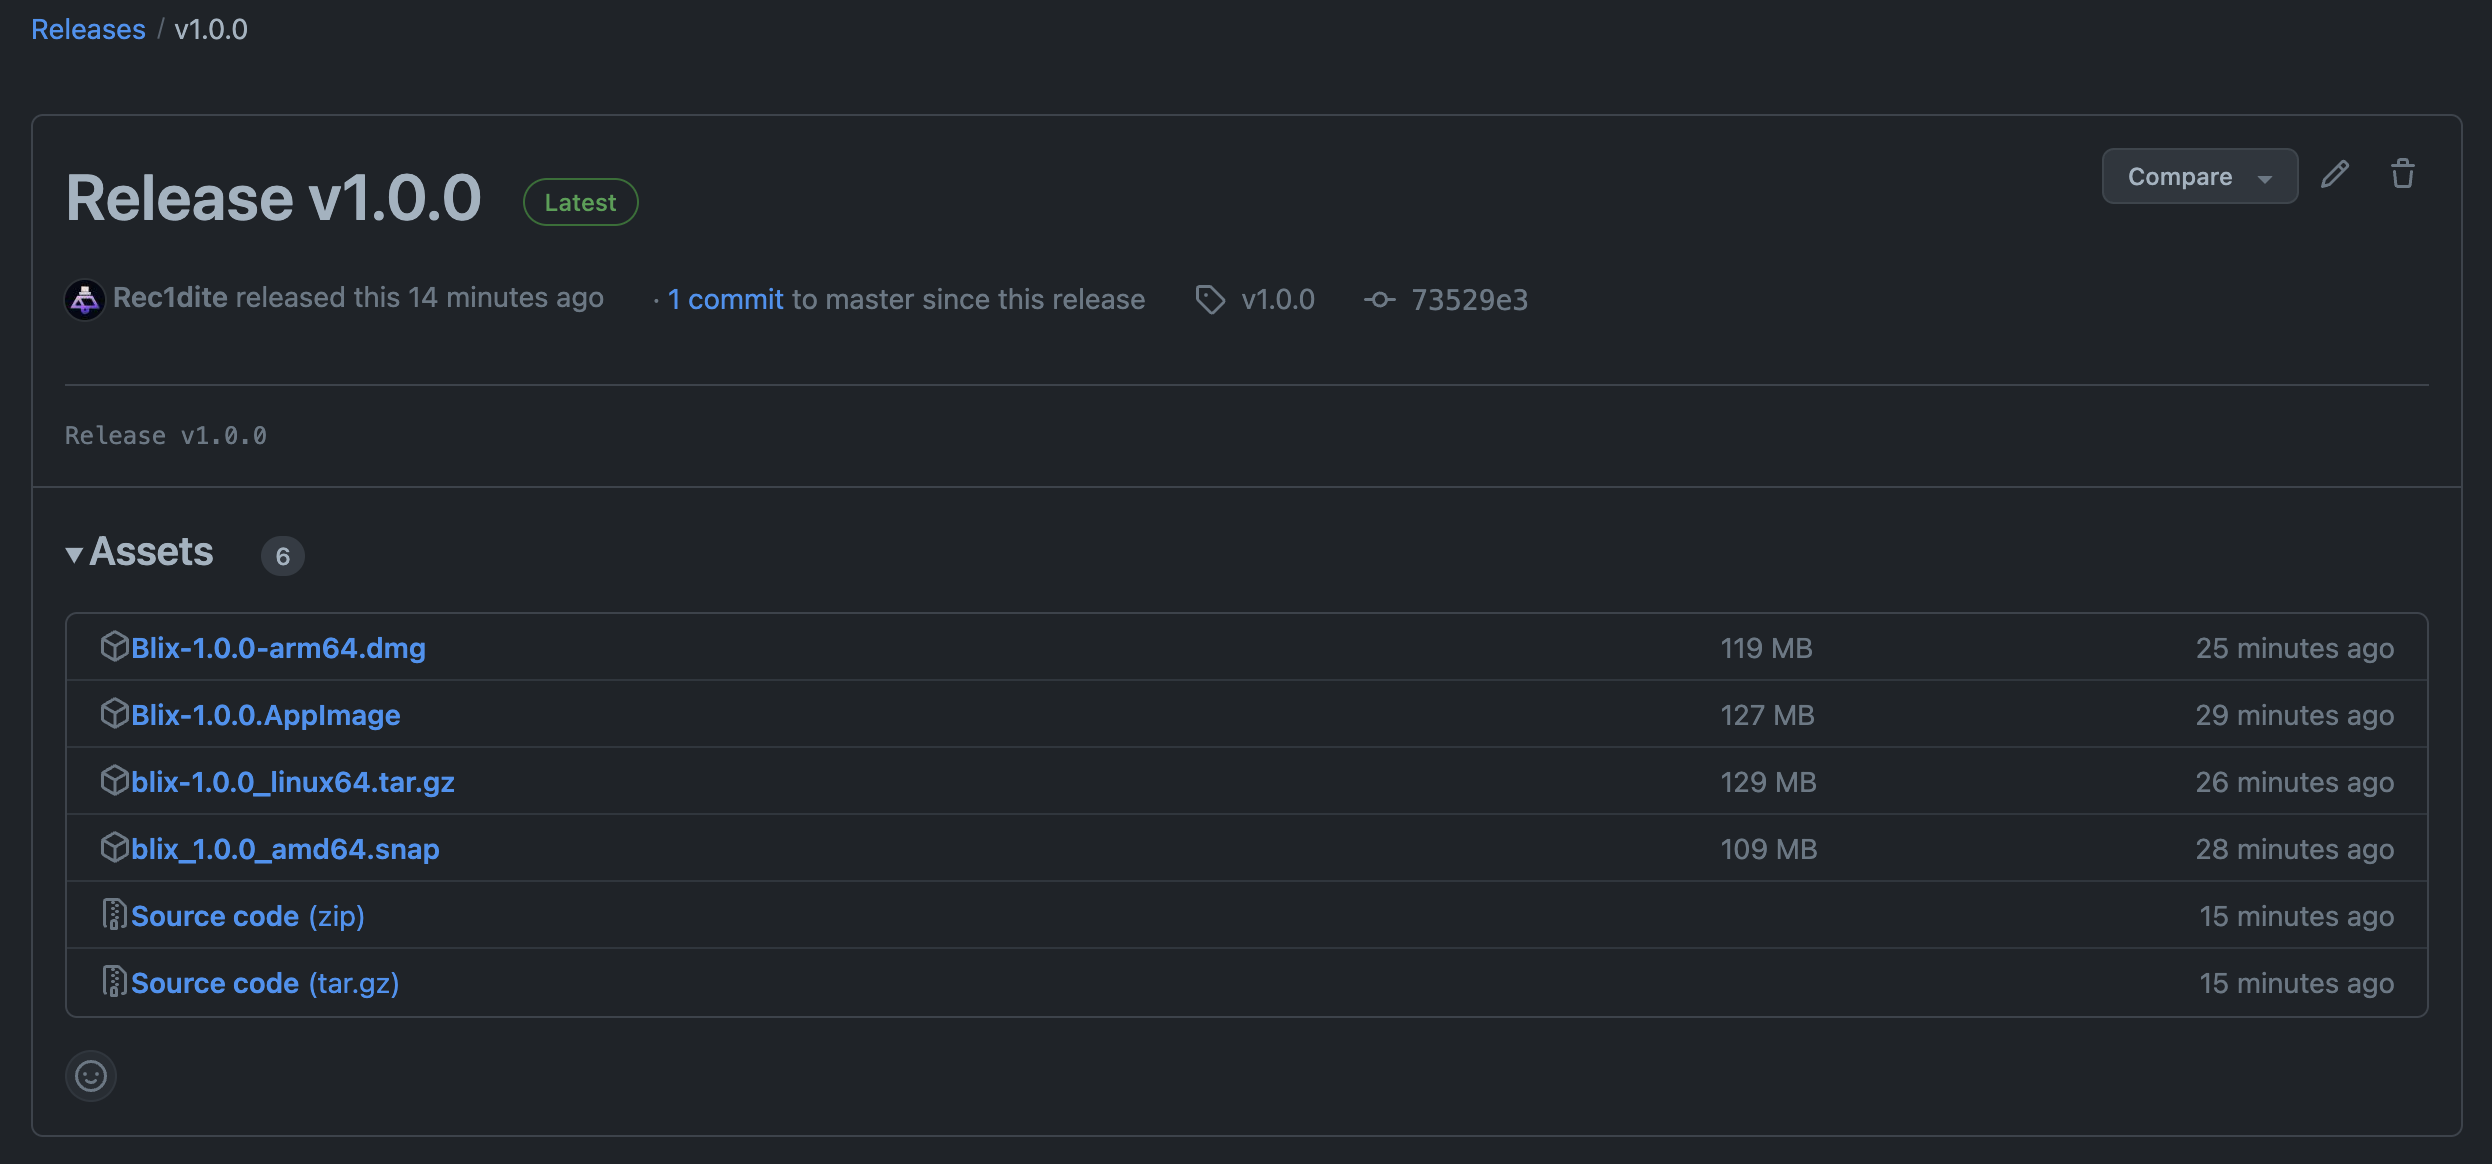
\includegraphics[width=1\textwidth,height=\textheight,keepaspectratio,rotate=0,origin=c]{../pics/github-release.png}
\end{figure}

\addcontentsline{toc}{subsection}{Linux}
\subsection*{Linux}

\begin{enumerate}[label*=\arabic*.]
	\item[\textbullet] {\bf Install Prerequisites}: 

	Open your Linux terminal and install \code{libvips} a requirement for
	image processing.

	\begin{lstlisting}[language=sh]
		sudo apt-get install libvips 
	\end{lstlisting}

	Then install the required python libraries to interact with the AI. Install
	\code{langchain} and \code{openai}. Python3 or higher is required.

	\begin{lstlisting}[language=sh]
		sudo apt install python3-pip
		pip3 install langchain
		pip3 install openai
	\end{lstlisting}

	\item[\textbullet] {\bf Download the app from GitHub releases for Linux}: 

	Download the \code{Blix-1.0.0.AppImage} file which includes Blix as a packed app.

	Open your Linux terminal again change directories to the same directory as
	where the app was downloaded. Then set the permissions of the app so that it can
	be executed as follows

	\begin{lstlisting}[language=sh]
		chmod +x Blix-1.0.0.AppImage
	\end{lstlisting}

	While in the same directory, launch the app as follows:

	\begin{lstlisting}[language=sh]
		./Blix-1.0.0.AppImage
	\end{lstlisting}
\end{enumerate}


\addcontentsline{toc}{subsection}{MacOS (Apple Silicon)}
\subsection*{MacOS (Apple Silicon)}


\begin{enumerate}[label*=\arabic*.]
	\item[\textbullet] {\bf Install Prerequisites}: 

	Open your terminal and install \code{libvips} a requirement for image
	processing. \code{Homebrew} is required to install it, if you don't have it
	installed on your machine then install it as follows first:

	\begin{lstlisting}[language=sh]
		 /bin/bash -c "$(curl -fsSL https://raw.githubusercontent.com/Homebrew/install/HEAD/install.sh)"
	\end{lstlisting}

	You may be prompted to enter your user password. The installation process
	will begin. Homebrew will download and install the necessary files. After it
	is installed run the following command to install \code{libvips}:

	\begin{lstlisting}[language=sh]
		brew install vips
	\end{lstlisting}

	Then install the required python libraries to interact with the AI. Install
	\code{langchain} and \code{openai}. Python3 or higher is required.

	\begin{lstlisting}[language=sh]
		brew install python
		pip3 install langchain
		pip3 install openai
	\end{lstlisting}

	\item[\textbullet] {\bf Download the app from GitHub releases for MacOS}: 

	Download the \code{Blix.1.0.0-arm64.dmg} file which includes Blix as a packed app.

	Go to the folder where the app was downloaded and then run the installation
	by double clicking the app.

	\begin{figure}[ht]
		\centering
		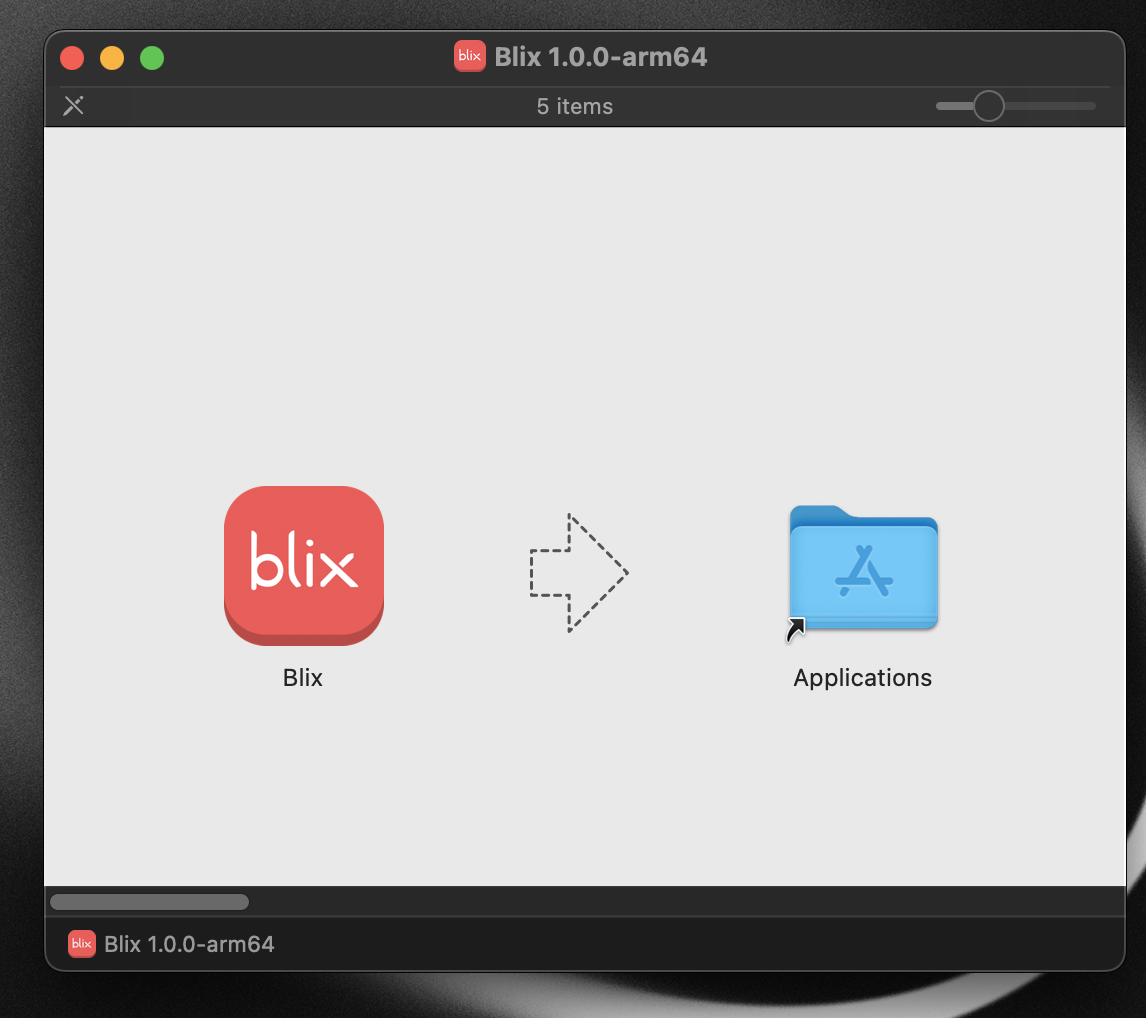
\includegraphics[width=0.3\textwidth,height=\textheight,keepaspectratio,rotate=0,origin=c]{../pics/mac-isntall.png}
	\end{figure}
\end{enumerate}

\addcontentsline{toc}{subsection}{Windows}
\subsection*{Windows}


\begin{enumerate}[label*=\arabic*.]
	\item[\textbullet] {\bf Install Prerequisites}: 

	You will need to install \textbf{libvips} for the image processing and compilation of the app.
	To install libvips on Windows, you can follow these steps:
\begin{enumerate}[label*=\arabic*.]
    \item[\textbullet]{Download libvips:}
	Go to the libvips releases page on GitHub: \url{https://github.com/libvips/libvips/releases}
        Scroll down to the "Assets" section of the latest release.
        Download the Windows installer package with a filename like vips-dev-w64-web-xxx.exe, where xxx represents the version number.
    \item[\textbullet]{Add libvips to the System Path:}
        After installation, you need to add the libvips binary directory to your system's PATH environment variable to make it accessible from the command line.
        Right-click on "This PC" (or "My Computer") and select "Properties."
        Click on "Advanced system settings" on the left sidebar.
        In the "System Properties" window, click on the "Environment Variables" button.
        Under the "System variables" section, find and select the "Path" variable, then click on "Edit."
        Click "New" and add the path to the libvips binary directory (usually something like \texttt{C:\textbackslash Program Files\textbackslash vips\textbackslash bin}).

    \item[\textbullet]{Test the Installation (Optional):}
        Open a new Command Prompt or PowerShell window.
        Type vips --version and press Enter. This should display the libvips version information if the installation was successful.
	\end{enumerate}

	\begin{lstlisting}[language=sh]
		 /bin/bash -c "$(curl -fsSL https://raw.githubusercontent.com/Homebrew/install/HEAD/install.sh)"
	\end{lstlisting}


	\item[\textbullet] {\bf Download the app from GitHub releases for Windows}: 

	Download the \code{Blix Setup 1.0.0.exe} file which is the installer for windows.

	Go to the folder where the app was downloaded and then run the installer
	by double clicking the app.

	The installer will automatically install blix on your device. 
	You can now simply click on the blix icon on your desktop to launch the app.

	% \begin{figure}[ht]
	% 	\centering
	% 	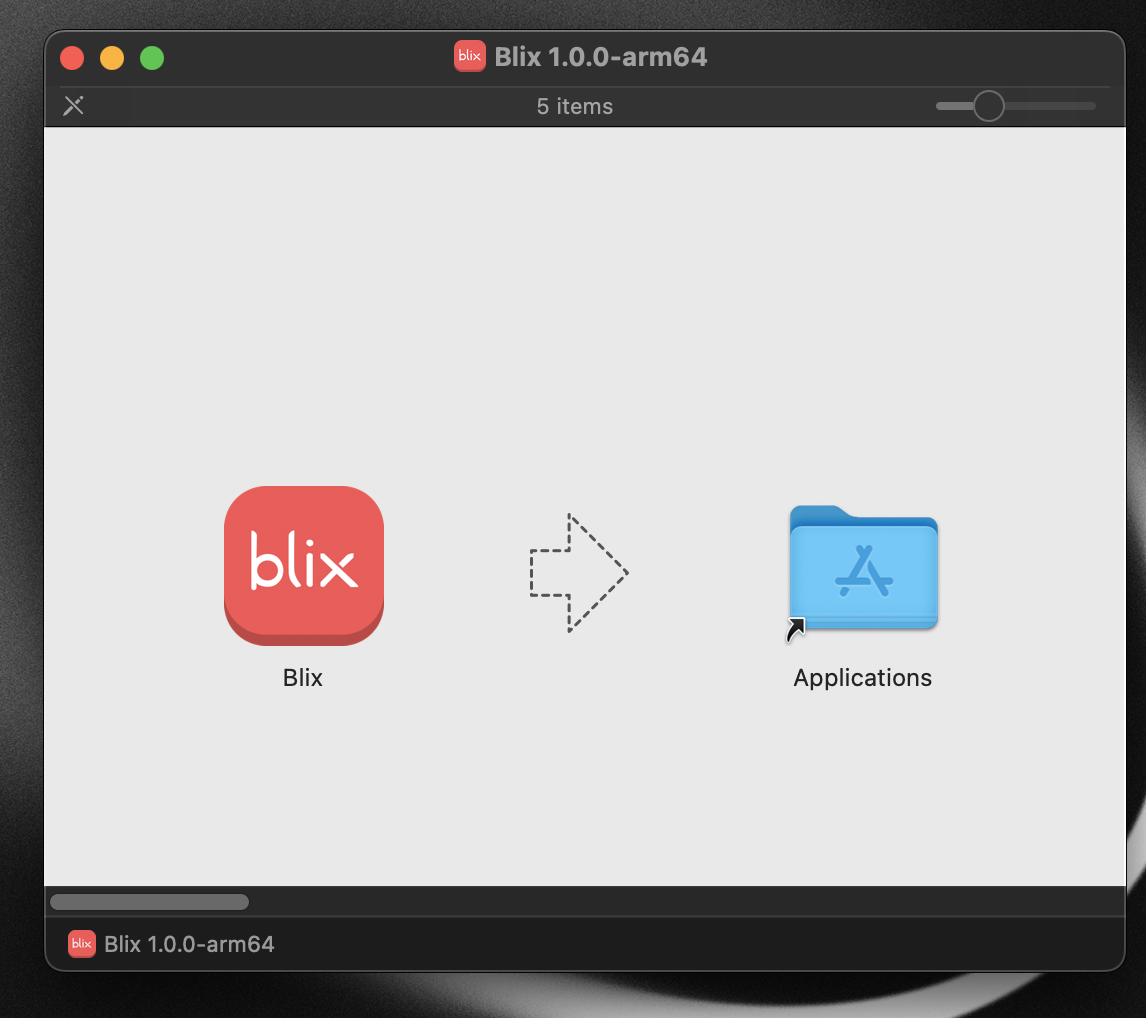
\includegraphics[width=0.3\textwidth,height=\textheight,keepaspectratio,rotate=0,origin=c]{../pics/mac-isntall.png}
	% \end{figure}
	% ADD WINDOWS IMAGE HERE
\end{enumerate}

\addcontentsline{toc}{section}{General Usage}
\section*{General Usage}

After installing and launching the app check the app you should see the
following home page as seen below. For detailed instructions for how to use the
app see our user manual.

\begin{figure}[ht]
	\centering
	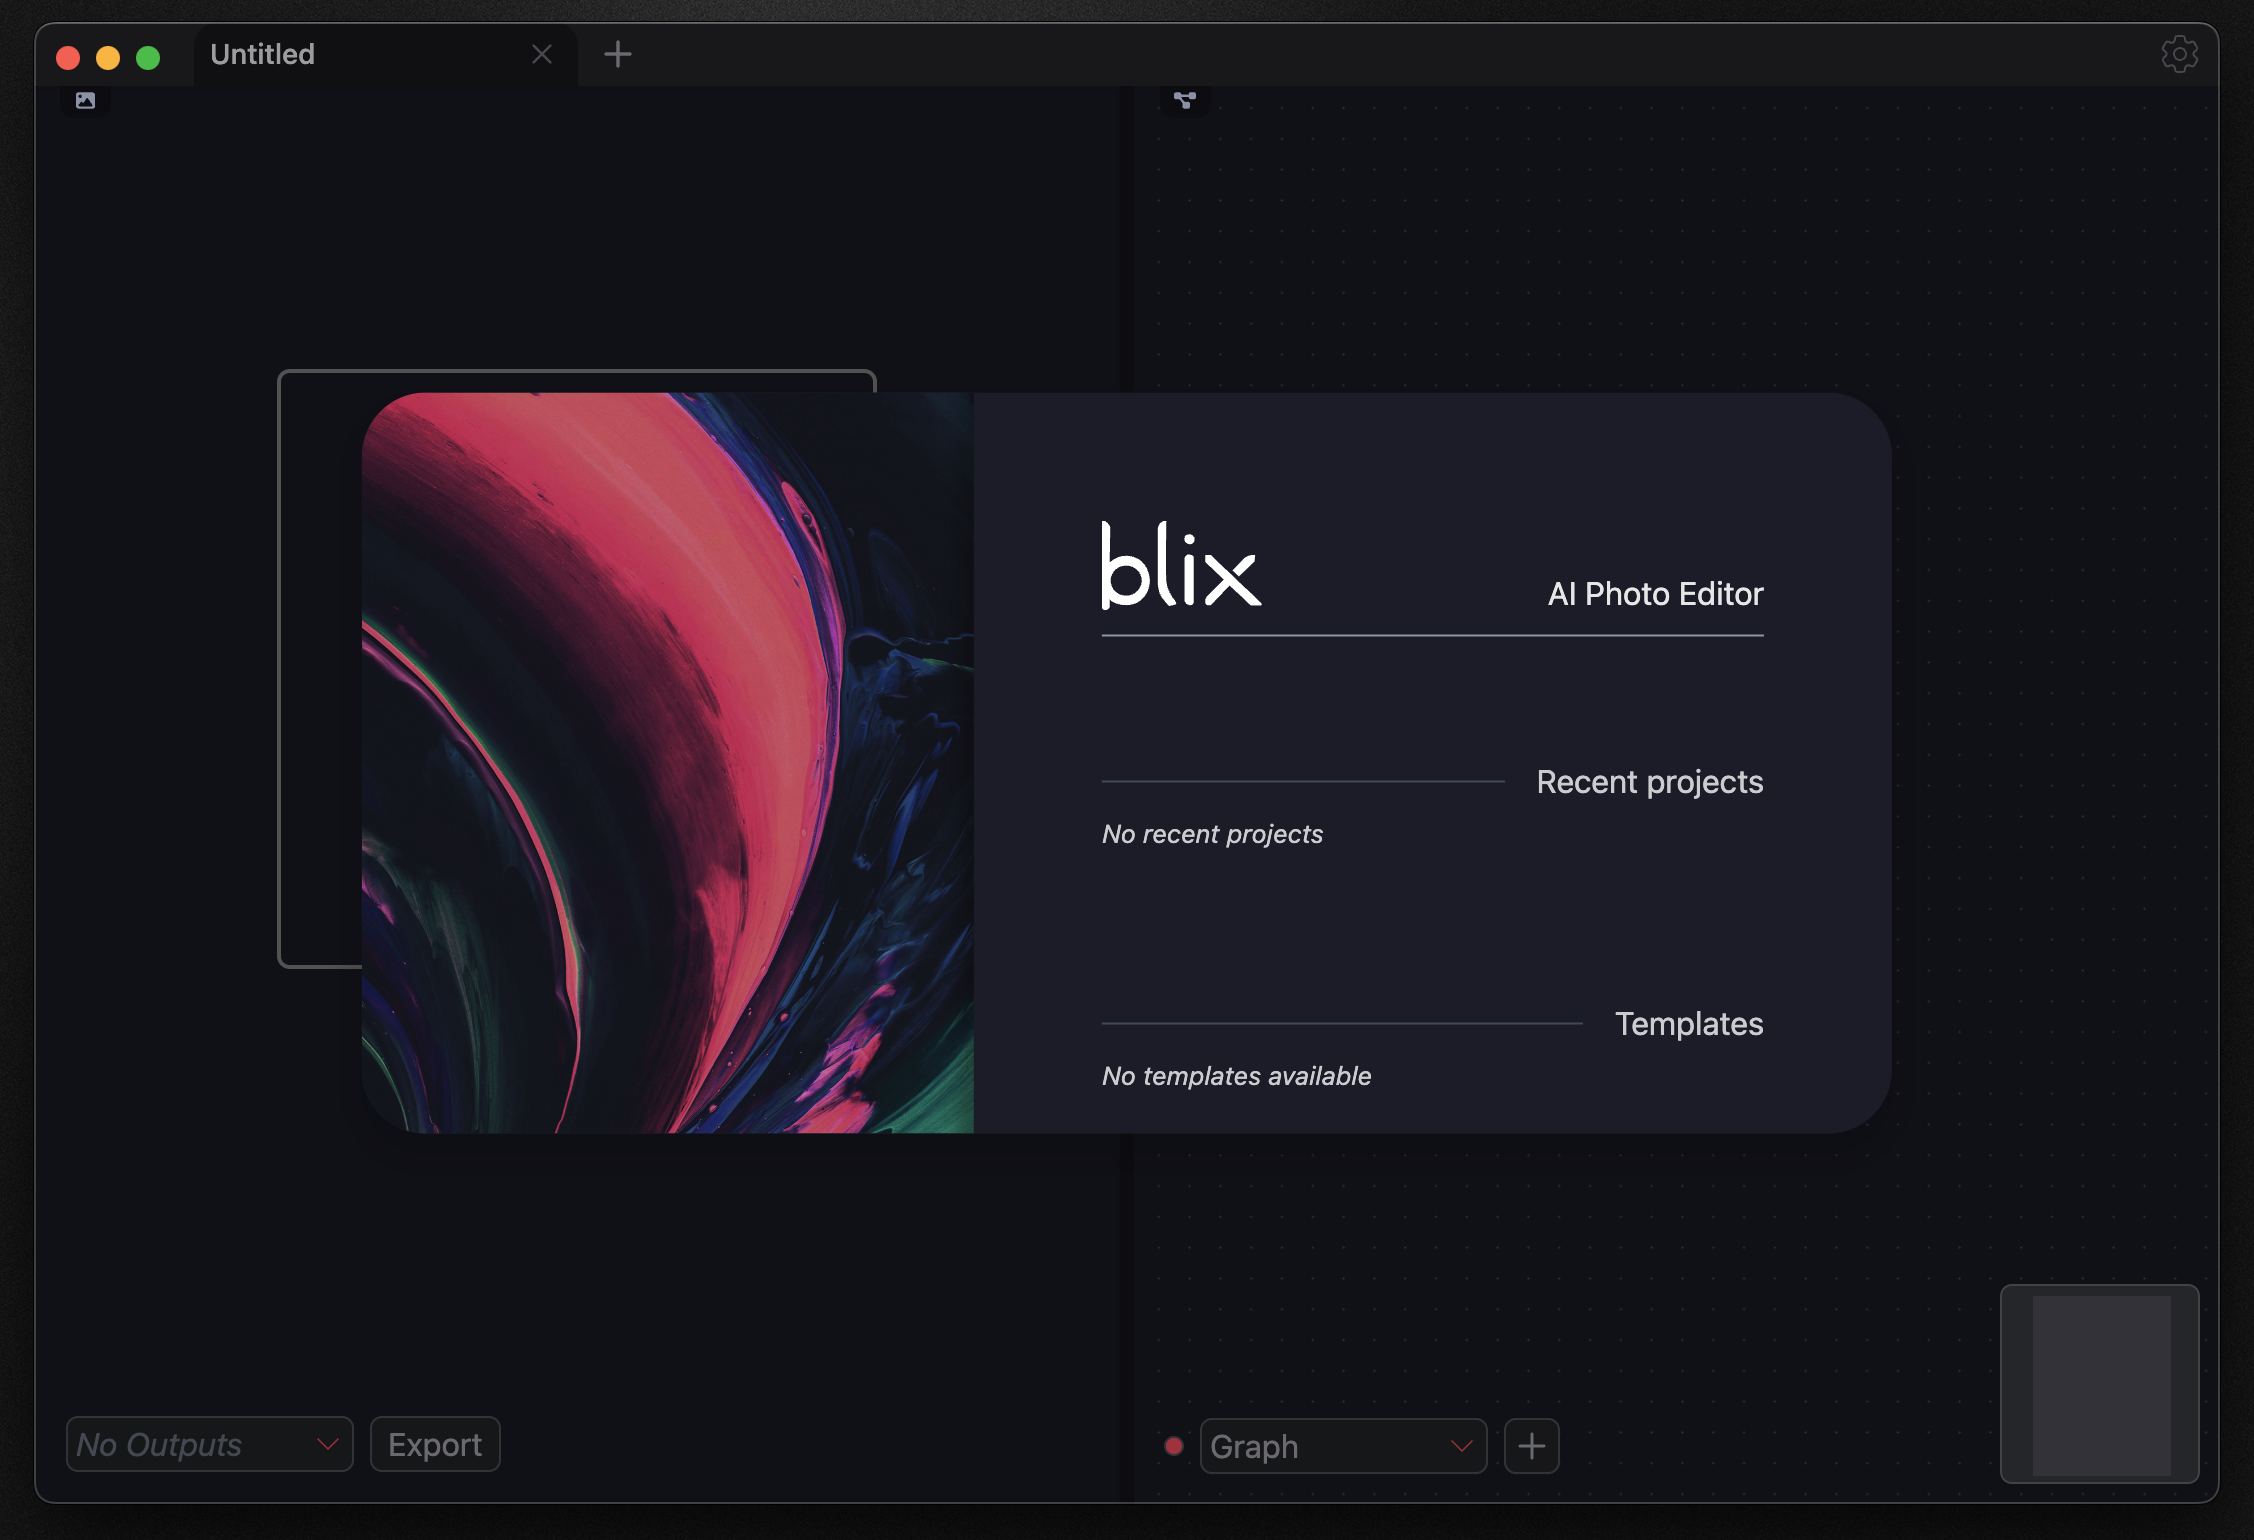
\includegraphics[width=1\textwidth,height=\textheight,keepaspectratio,rotate=0,origin=c]{../pics/blix-homepage.png}
\end{figure}




\end{document}